\documentclass[crop, tikz]{standalone}
\usepackage{tikz}

\usetikzlibrary{calc}
\usepackage{colortbl}

 
 
\begin{document}
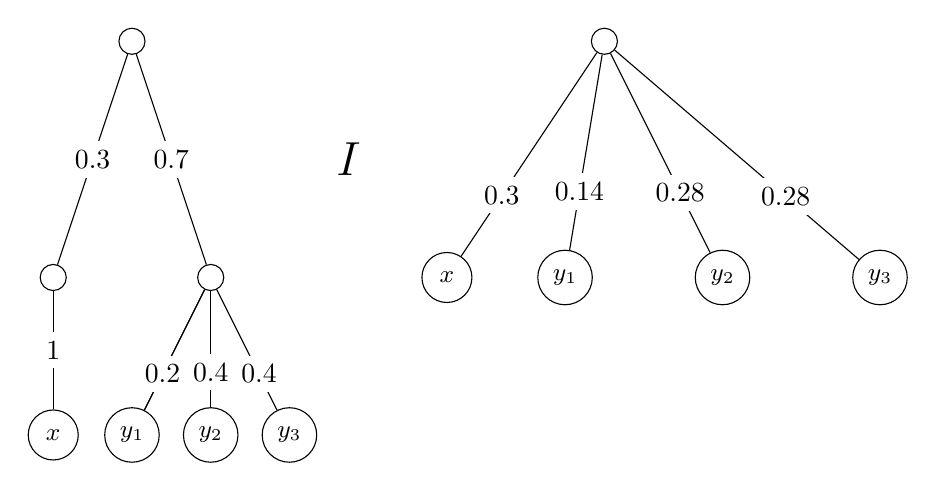
\begin{tikzpicture}[scale=1]
	% Axis
%%itikz


   \node[draw,circle] (l1_0) at (-1,3) {$ $};
   \node[draw,circle] (l1_1) at (-2,0) {$ $};
   
      \node[draw,circle, minimum width=0.25in] (l2_1) at (-2,-2) {\small $x$};

   \node[draw,circle] (l1_2) at (0,0) {$ $};
      \path[draw] (l1_1) to node[fill=white] {$1$} (l2_1);

      \node[draw,circle, minimum width=0.25in] (l2_1) at (-1,-2) {\small $y_1$};
      \node[draw,circle, minimum width=0.25in] (l2_2) at (0,-2) {\small $y_2$};
      \node[draw,circle, minimum width=0.25in] (l2_3) at (1,-2) {\small $y_3$};

   \path[draw] (l1_2) to[pos=0.7]  node[fill=white] {$1$} (l2_1);

   \path[draw] (l1_0) to node[fill=white] {$0.3$} (l1_1);
   \path[draw] (l1_0) to node[fill=white] {$0.7$} (l1_2);

   \path[draw] (l1_2) to[pos=0.7]  node[fill=white] {$0.2$} (l2_1);
   \path[draw] (l1_2) to[pos=0.7]  node[fill=white] {$0.4$} (l2_2);
   \path[draw] (l1_2) to[pos=0.7]  node[fill=white] {$0.4$} (l2_3);

\node at (1.75,1.5) {\LARGE $I$};

   \node[draw,circle] (l2_0) at (5,3) {$ $};
   \node[draw,circle, minimum width=0.25in] (l2_1) at (3,0) {\small $x$};
   \node[draw,circle, minimum width=0.25in] (l2_2) at (4.5,0) {\small $y_1$};
   \node[draw,circle, minimum width=0.25in] (l2_3) at (6.5,0) {\small $y_2$};
   \node[draw,circle, minimum width=0.25in] (l2_4) at (8.5,0) {\small $y_3$};
   
   \path[draw] (l2_0) to[pos=0.7]  node[fill=white] {$0.3$} (l2_1);
   \path[draw] (l2_0) to[pos=0.7] node[fill=white] {$0.14$} (l2_2);
   \path[draw] (l2_0) to[pos=0.7] node[fill=white] {$0.28$} (l2_3);
   \path[draw] (l2_0) to[pos=0.7] node[fill=white] {$0.28$} (l2_4);


   \end{tikzpicture}

 \end{document}
